\section{Conclusion}\label{sec:conclusion}

This proposal puts forth a novel program to uncover the origins of dark matter
by searching for evidence of strongly coupled dark sectors or ``dark QCD''
using the Compact Muon Solenoid (CMS) experiment at the Large Hadron Collider (LHC).
The program is complementary to other ongoing efforts:
direct detection and annihilation experiments have highly suppressed sensitivity to these models.
Previous collider searches have overlooked their novel phenomenological signatures,
including semivisible jets, emerging jets, and soft unclustered energy patterns.
Expanding on the initial explorations in the LHC Run 2 dataset,
we will conduct a unified search for semivisible jets by increasing the model independence at every stage,
employing the latest unsupervised artificial intelligence (AI) techniques.
\textbf{LHC Run 3 offers an unparalleled opportunity for model-independent data collection and analysis.}
Finally, we will conduct the first scan of all dark QCD models, including combinations of the new phenomena,
to identify unconstrained signatures and design the next steps in the program for the upcoming HL-LHC.

\textbf{We will deliver the substantial quantities of simulated events required for this program
by developing fast and accurate detector simulation using generative AI.}
Using cutting-edge diffusion models and applying the latest acceleration techniques,
we will generate particle showers at least 100 times faster than the CPU-based full detector simulation.
The algorithms will be deployed on coprocessors across the computing grid using inference as a service,
the most efficient and portable approach.
In addition to enabling the dark QCD scan over the entire model space,
AI-based simulation will resolve a major computing challenge for the high luminosity LHC upgrade.
The same techniques, in combination with new GPU-based classical simulation engines,
will push forward the design of the future muon collider and its detector systems
by simulating the beam-induced background (BIB) from muon decays in flight.

The PI is uniquely suited to deliver both aspects of the proposal.
His expertise and leadership in dark QCD, AI algorithms, detector simulation, inference on coprocessors, and experiment software are widely recognized.
As a Fermilab scientist, he can leverage the lab's AI, computing, and theory expertise and direct the lab's facilities to ensure success.
The results will significantly advance the mission of the DOE Office of Science to search for physics beyond the standard model and to capitalize on national computing resources.
\textbf{The methods and products from this proposal will benefit not just the energy frontier, but also the neutrino and cosmic frontiers.}

\subsection{Timetable of Activities and Deliverables}

Figure~\ref{fig:activities} summarizes the steps, contributors, and deliverables in each part of the proposal (Sections~\ref{sec:darkqcd} and~\ref{sec:ml4sim}).
Budget years (BYs) 1 and 2 correspond to the remaining years of LHC Run 3, while BY5 corresponds to the final year of the long shutdown before HL-LHC operations commence.
The last two budget years are devoted to the final, most ambitious deliverables: the dark QCD scan and future collider simulation.
The deliverables include new dark QCD models in BY2, at least one limited-author AI algorithm publication and the Run 3 semivisible jet search publication in BY3, and the full dark QCD scan publication in BY5.
On the technical side, we will deliver the AI-based simulation for CMS in BY3 and for the muon collider in BY5, with corresponding publications.

The PI and postdoctoral research associate (RA) will co-lead both the dark QCD searches and the AI-based simulation development.
Their effort will be supplemented by two AI associates (AIAs).
AIA\#1 will focus on the optimization of AI algorithms for jet tagging, jet mass, and diffusion during BYs 2--3.
AIA\#2 will implement the AI-based simulation in the experiment software framework using inference as a service during BYs 4--5, ensuring its scalability and smooth operation in high performance computing sites.
This distribution of personpower ensures maximal effort is available leading up to and during BY3, when several deliverables are expected.

\begin{figure}[htb!]
\centering
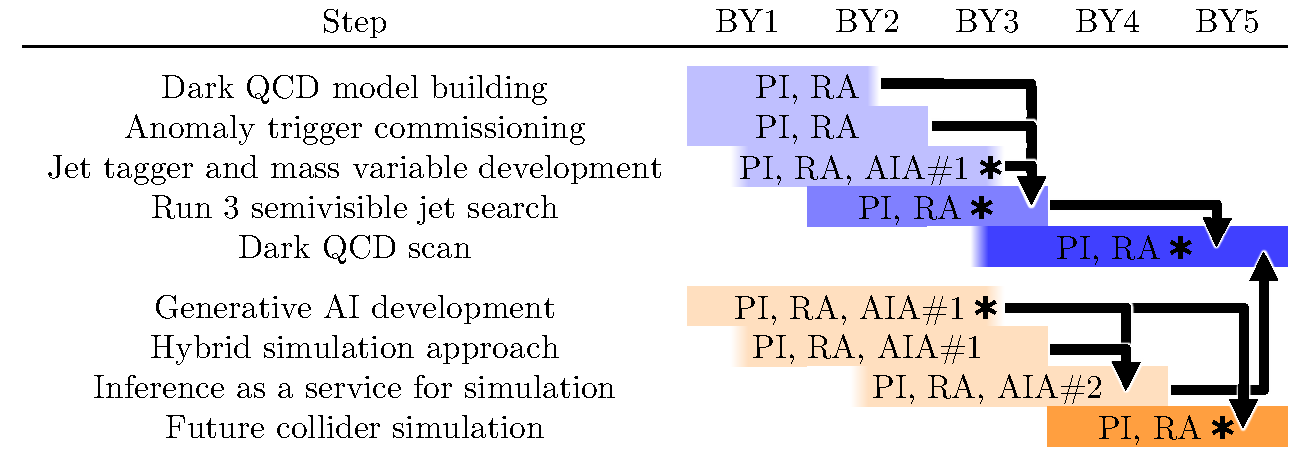
\includegraphics[width=0.95\myfigurewidth]{figures/table_final.pdf}
\caption{A summary of the steps in the strongly coupled dark matter searches and fast detector simulation development in each budget year. The contributions of the PI, RA, and AIAs are noted. The symbol $\ast$ indicates an expected publication. Arrows indicate dependencies between steps.}
\label{fig:activities}
\end{figure}

\clearpage
